\documentclass[11pt,answers]{exam}
\usepackage[spanish]{babel}
\usepackage[utf8]{inputenc}
\usepackage[T1]{fontenc}
\usepackage{amsmath,amssymb,amsfonts}
\usepackage{graphicx}
\usepackage{colortbl}
\usepackage{xcolor}
\usepackage{multirow}
\usepackage{float}
\usepackage{enumitem}
\usepackage{algorithm}
\usepackage{mathrsfs}
\usepackage{array} % Para controlar el ancho de las celdas
\usepackage{enumitem} % Para personalizar listas
\usepackage{listings}% http://ctan.org/pkg/listings
\usepackage{hyperref} % for hyperlinks
\usepackage{amsmath} % para matemáticas mejoradas
\usepackage{algorithm} % para escribir pseudocódigos
\usepackage{algpseudocode} % para escribir pseudocódigos
\usepackage[version=4]{mhchem}
\usepackage{stmaryrd}

% \usepackage{etoolbox}

% \AtBeginEnvironment{align}{\setcounter{equation}{0}}

\renewcommand{\solutiontitle}{\noindent\textbf{Solución:}\par\noindent}

\lstset{
  basicstyle=\ttfamily,
  mathescape
}

\graphicspath{{public/}}

\setlength{\topmargin}{-.5in} \setlength{\textheight}{9.25in}
\setlength{\oddsidemargin}{-0.5in} \setlength{\textwidth}{7.2in}


\begin{document}
\begin{center}
    \newcommand{\HRule}{\rule{\linewidth}{0.5mm}}
    \begin{minipage}{0.48\textwidth} 
        \begin{flushleft}
            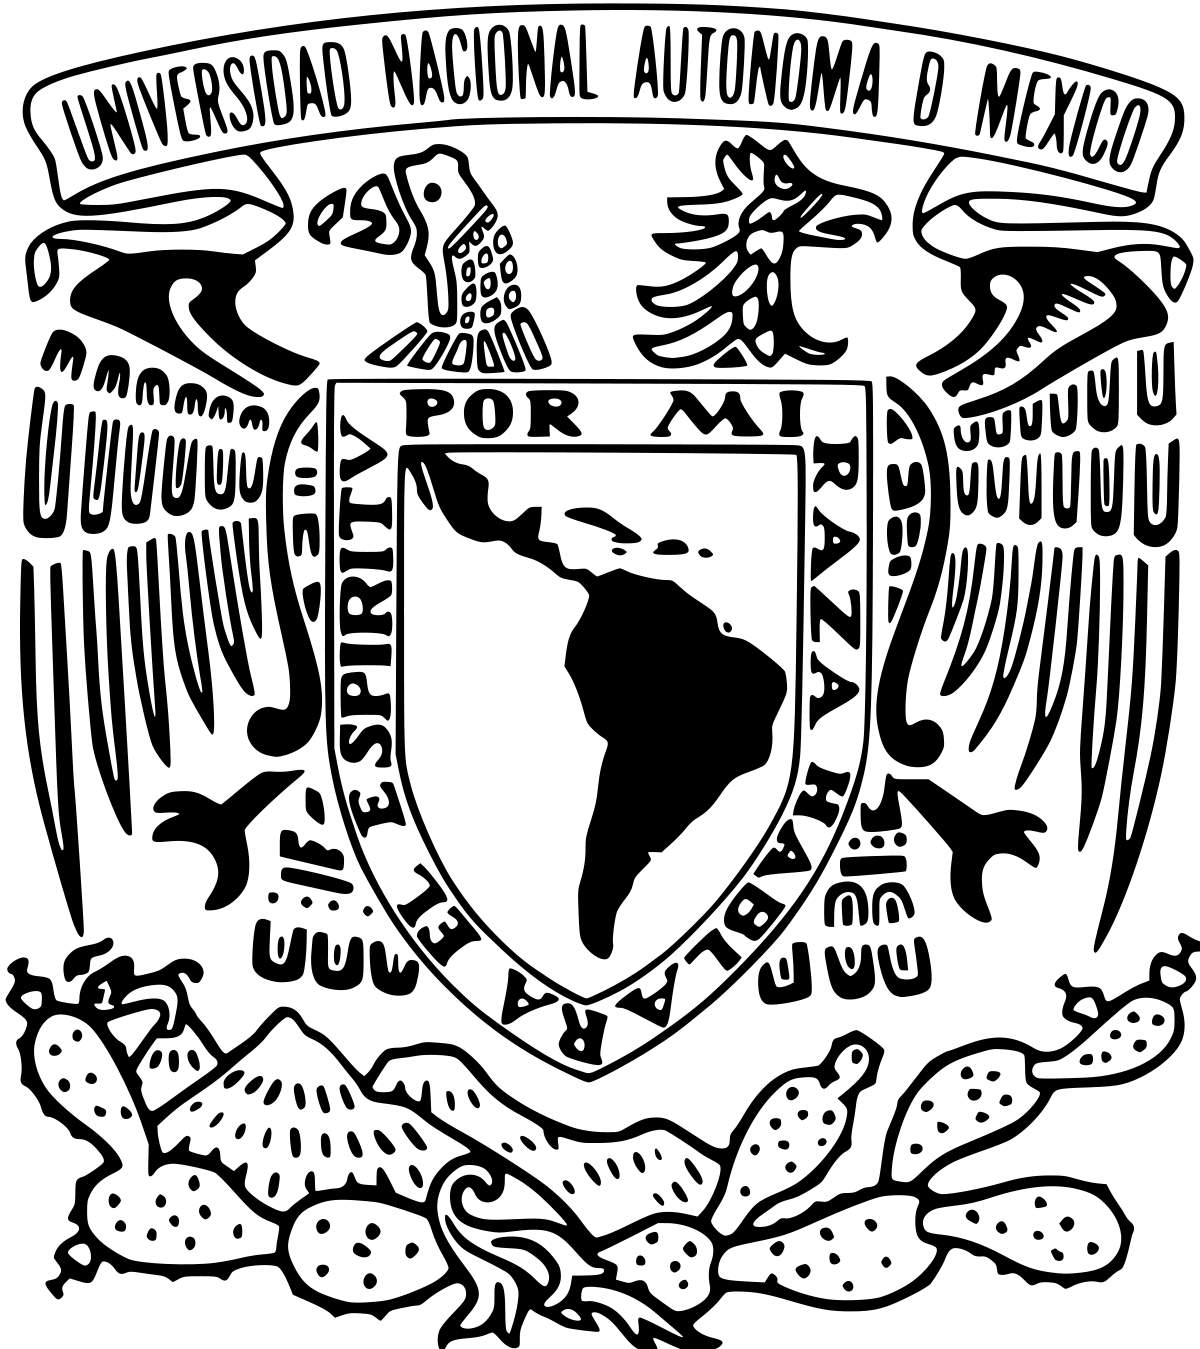
\includegraphics[scale = 0.08]{../../../public/logo_unam.png}
        \end{flushleft}
    \end{minipage}
    \begin{minipage}{0.48\textwidth} 
        \begin{flushright}
            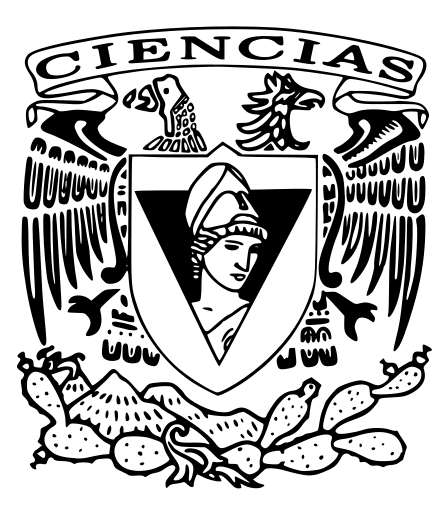
\includegraphics[scale =0.22]{../../../public/logo_ciencias.png}
        \end{flushright}
    \end{minipage}
    \vspace*{-1.5cm}						
    \textsc{\huge Nacional Autónoma de México \\ \vspace{-4px} Universidad }\\[2cm]	
    \textsc{\LARGE Facultad de Ciencias}\\[1.5cm]
    \vspace*{1cm}					
        \HRule \\[0.7cm]							
            { \huge \bfseries Tarea 03}\\[0.4cm]	
        \HRule \\[1.5cm]						    
    \begin{minipage}{0.52\textwidth}													
        \begin{flushleft} \large	
            \small
            \vspace{-0.6cm}	
            \vspace{-0.6cm}	
                \emph{Alumno:}\\
               Ramírez López Alvaro. 316276355\\
            \vspace*{2cm}
        \end{flushleft}																		
        \end{minipage}		
    \begin{minipage}{0.46\textwidth}		
        \vspace{-0.6cm}											
        \begin{flushright} \large						
            \small										
            \emph{Profesor:} Jesús Villagómez Chávez	\\
            \emph{Ayudantes:}
                Gabriela Peña Franco	 \\
                Martha Rubí Gutiérrez González	 \\
        \end{flushright}																
    \end{minipage}	
    \vspace*{1cm}
    \vspace{2cm}
    \begin{center}						
        {\large 9 de septiembre de 2024}
    \end{center}  						
\end{center}	
\textbf{}
\newpage

\begin{enumerate}
    \item Construye un lenguaje formal adecuado para que se pueda escribir los siguientes conceptos. Exhibe la fórmula que hace expresable el concepto en el lenguaje.
    \begin{enumerate}
        \item El orden en el conjunto de los números racionales.
        \item Que una función sea monótona.
        \item Que una relación sea de equivalencia.
        \item Tener exactamente tres elementos.
        \item Nadie en la clase de conjuntos es más inteligente que todos en la clase de lógica.
    \end{enumerate}

    \begin{solution}
    \begin{enumerate}
    \item \textbf{El orden en el conjunto de los números racionales} \\
    Utilizamos una relación binaria \( < \) que representa el orden en los números racionales, denotados por \( \mathbb{Q} \). La fórmula en lógica de primer orden es:
    \[
    \forall x, y, z \in \mathbb{Q}, (x < y \land y < z \rightarrow x < z) \land (x < y \rightarrow \neg(y < x))
    \]

    \item \textbf{Que una función sea monótona} \\
    Sea \( f: A \rightarrow B \) una función. La monotonía de una función se puede expresar como:
    \[
    \forall x, y \in A, (x \leq y \rightarrow f(x) \leq f(y))
    \]

    \item \textbf{Que una relación sea de equivalencia} \\
    Sea \( R \) una relación sobre un conjunto \( A \). La relación \( R \) es de equivalencia si es reflexiva, simétrica y transitiva:
    \[
    \text{Reflexiva:} \quad \forall x \in A, R(x, x)
    \]
    \[
    \text{Simétrica:} \quad \forall x, y \in A, (R(x, y) \rightarrow R(y, x))
    \]
    \[
    \text{Transitiva:} \quad \forall x, y, z \in A, (R(x, y) \land R(y, z) \rightarrow R(x, z))
    \]

    \item \textbf{Tener exactamente tres elementos} \\
    Sea \( A \) un conjunto. Para expresar que \( A \) tiene exactamente tres elementos:
    \[
    \exists x, y, z \in A, (x \neq y \land x \neq z \land y \neq z \land \forall w \in A, (w = x \lor w = y \lor w = z))
    \]

    \item \textbf{Nadie en la clase de conjuntos es más inteligente que todos en la clase de lógica} \\
    Supongamos que \( C \) es la clase de conjuntos, \( L \) es la clase de lógica, y \( I(x, y) \) indica que \( x \) es más inteligente que \( y \). La fórmula es:
    \[
    \forall x \in C, \exists y \in L, \neg I(x, y)
    \]
\end{enumerate}
\end{solution}
    
    \item Verifica si las siguientes fórmulas son teoremas del cálculo de proposiciones o no. Si la respuesta es afirmativa, da la prueba.
    \begin{enumerate}
        \item $\alpha \to (\alpha \to \alpha)$
        \item $(\alpha \to \alpha) \to \alpha$
        \item $(\neg \alpha \to \beta) \to (\neg \beta \to \neg \alpha)$
        \item $(\alpha \to \gamma) \to (\neg \alpha \to \beta)$
    \end{enumerate}

    \begin{solution}
% \begin{enumerate}
%     \item \( \alpha \to (\alpha \to \alpha) \) \\
%     \textbf{Prueba:} \\
%     Usamos el \textbf{Axioma 1}: \( A \to (B \to A) \). \\
%     Sustituimos \( A \) por \( \alpha \) y \( B \) por \( \alpha \), obteniendo:
%     \[
%     \alpha \to (\alpha \to \alpha)
%     \]
%     Por lo tanto, esta fórmula \textbf{es un teorema} del cálculo proposicional.

%     \item \( (\alpha \to \alpha) \to \alpha \) \\
%     \textbf{Prueba:} \\
%     No parece posible derivar \( (\alpha \to \alpha) \to \alpha \) directamente a partir de los axiomas proporcionados. Esta fórmula no es válida en general, ya que suponer que \( \alpha \to \alpha \) implica \( \alpha \) no es siempre cierto. \\
%     Por lo tanto, esta fórmula \textbf{no es un teorema} del cálculo proposicional.

%     \item \( (\neg \alpha \to \beta) \to (\neg \beta \to \neg \alpha) \) \\
%     \textbf{Prueba:} \\
%     Utilizamos el \textbf{Axioma 3}: \( (\neg B \to \neg A) \to ((\neg B \to A) \to A) \). \\
%     Hacemos la sustitución de variables: \( B = \beta \) y \( A = \alpha \), obteniendo:
%     \[
%     (\neg \beta \to \neg \alpha) \to ((\neg \beta \to \alpha) \to \alpha)
%     \]
%     Esta fórmula muestra una estructura relacionada con la contraposición. Además, el teorema \( (\neg \alpha \to \beta) \to (\neg \beta \to \neg \alpha) \) es un teorema clásico conocido como \textit{contraposición}. \\
%     Por lo tanto, esta fórmula \textbf{sí es un teorema} del cálculo proposicional.

%     \item \( (\alpha \to \gamma) \to (\neg \alpha \to \beta) \) \\
%     \textbf{Prueba:} \\
%     No parece posible derivar esta fórmula directamente utilizando los tres axiomas dados. No hay una conexión clara entre \( \alpha \to \gamma \) y \( \neg \alpha \to \beta \). \\
%     Por lo tanto, esta fórmula \textbf{no es un teorema} del cálculo proposicional.
% \end{enumerate}
\end{solution}
    
    \item Asume que $N$ denota ’es un número’, $I$ denota ’es interesante’, y $c_0$ denota el símbolo de constante cero. Traduce las siguientes frases a un lenguaje lógico. Si la frase es ambigua, necesitará más de una traducción:
    \begin{enumerate}
        \item El cero es el menor de todos los números.
        \item Si cualquier número es interesante, entonces el cero es interesante.
        \item Ningún número es menor que el cero.
        \item Cualquier número no interesante con la propiedad de que todo número menor que dicho número sea interesante vuelve a este número interesante.
        \item No hay un número tal que todos los demás números sean menores que éste.
        \item No hay un número tal que ningún otro número sea menor que él.
    \end{enumerate}

    \begin{solution}
    \begin{itemize}
    \item El cero es el menor de todos los números.
    \begin{itemize}
        \item Traducción 1: \( \forall x (N(x) \rightarrow c_0 \leq x) \)
    \end{itemize}
    
    \item Si cualquier número es interesante, entonces el cero es interesante.
    \begin{itemize}
        \item Traducción: \( (\forall x (N(x) \rightarrow I(x))) \rightarrow I(c_0) \)
    \end{itemize}
    
    \item Ningún número es menor que el cero.
    \begin{itemize}
        \item Traducción: \( \forall x (N(x) \rightarrow \neg <(x, c_0)) \)
    \end{itemize}
    
    \item Cualquier número no interesante con la propiedad de que todo número menor que dicho número sea interesante vuelve a este número interesante.
    \begin{itemize}
        \item Traducción: \( \forall x ((N(x) \land \neg I(x) \land \forall y (<(y, x) \rightarrow I(y))) \rightarrow I(x)) \)
    \end{itemize}
    
    \item No hay un número tal que todos los demás números sean menores que éste.
    \begin{itemize}
        \item Traducción: \( \neg \exists x (N(x) \land \forall y (N(y) \rightarrow <(y, x))) \)
    \end{itemize}
    
    \item No hay un número tal que ningún otro número sea menor que él.
    \begin{itemize}
        \item Traducción: \( \neg \exists x (N(x) \land \forall y (N(y) \rightarrow \neg <(y, x))) \)
    \end{itemize}
\end{itemize}

\end{solution}
    
    \item Con la misma notación del ejercicio anterior, traduce al español la siguiente fórmula:
    \[
    \forall x ((N(x) \to I(x)) \to \neg \forall y ((N(y) \to I(y)) \to \neg (x < y)))
    \]
    \begin{solution}
    La traducción al español sería:

    \textit{Para todo $x$, si $x$ es un número, entonces $x$ es interesante; lo cual implica que no es cierto que para todo $y$, si $y$ es un número, entonces $y$ es interesante y no es cierto que $x$ sea menor que $y$.}


\end{solution}

    \item Sean $L$ un lenguaje formal, $\mathscr{R}$ una colección de reglas de inferencia y $\Gamma$, $\Delta$ colecciones de fórmulas. Demuestra que $\overline{\Gamma \cap \Delta} \subseteq \overline{\Gamma} \cap \overline{\Delta}$.
    \begin{solution}
\textbf{Demostración:}

Sea $\overline{X}$ el conjunto de todas las consecuencias lógicas de una colección $X$ de fórmulas, es decir, 
\[
\overline{X} = \{ \varphi \mid \Gamma \vdash \varphi \}.
\]
Queremos demostrar que 
\[
\overline{\Gamma \cap \Delta} \subseteq \overline{\Gamma} \cap \overline{\Delta}.
\]

Supongamos que $\varphi \in \overline{\Gamma \cap \Delta}$. Esto significa que existe una deducción de $\varphi$ a partir de las fórmulas en $\Gamma \cap \Delta$ utilizando las reglas de inferencia de $\mathscr{R}$. Es decir,
\[
\Gamma \cap \Delta \vdash \varphi.
\]
Dado que $\Gamma \cap \Delta \subseteq \Gamma$, esto implica que también podemos deducir $\varphi$ a partir de las fórmulas en $\Gamma$, es decir,
\[
\Gamma \vdash \varphi,
\]
lo que significa que $\varphi \in \overline{\Gamma}$.

De manera similar, dado que $\Gamma \cap \Delta \subseteq \Delta$, también podemos deducir $\varphi$ a partir de las fórmulas en $\Delta$, es decir,
\[
\Delta \vdash \varphi,
\]
lo que significa que $\varphi \in \overline{\Delta}$.

Por lo tanto, tenemos que $\varphi \in \overline{\Gamma}$ y $\varphi \in \overline{\Delta}$, lo que implica que 
\[
\varphi \in \overline{\Gamma} \cap \overline{\Delta}.
\]
En consecuencia, hemos demostrado que 
\[
\overline{\Gamma \cap \Delta} \subseteq \overline{\Gamma} \cap \overline{\Delta}.
\]
\qed

\end{solution}

    \item Sean $L$ un lenguaje formal, $\mathscr{R}$ una colección de reglas de inferencia, $\Gamma$ una colección de fórmulas y $A$ es una fórmula. Demuestra que las siguientes condiciones son equivalentes:
    \begin{enumerate}
        \item $\Gamma$ es una teoría (formal).
        \item $\Gamma \vdash A$ si y sólo si $A \in \Gamma$.
    \end{enumerate}
    \begin{solution}
Sean $L$ un lenguaje formal, $\mathscr{R}$ una colección de reglas de inferencia, $\Gamma$ una colección de fórmulas y $A$ es una fórmula. Demuestra que las siguientes condiciones son equivalentes:
    \begin{enumerate}
        \item $\Gamma$ es una teoría (formal).
        \item $\Gamma \vdash A$ si y sólo si $A \in \Gamma$.
    \end{enumerate}

\textbf{Demostración:}

Queremos demostrar que las dos condiciones son equivalentes.

\begin{itemize}
    \item[$\Rightarrow$] Supongamos que $\Gamma$ es una teoría formal. Por la definición de teoría, sabemos que $\Gamma$ es deductivamente cerrada, es decir, para toda fórmula $A$, si $\Gamma \vdash A$, entonces $A \in \Gamma$. Esto implica que, si $A$ es deducible a partir de $\Gamma$, entonces $A$ ya pertenece a $\Gamma$, lo cual muestra la implicación directa de que $\Gamma \vdash A$ implica $A \in \Gamma$.

    Además, por definición de teoría, si una fórmula $A$ pertenece a $\Gamma$, entonces también es deducible de $\Gamma$ usando las reglas de inferencia $\mathscr{R}$, es decir, $A \in \Gamma$ implica $\Gamma \vdash A$. Esto demuestra la implicación inversa, es decir, si $A \in \Gamma$, entonces $\Gamma \vdash A$.

    Por lo tanto, hemos demostrado que $\Gamma \vdash A$ si y sólo si $A \in \Gamma$.

    \item[$\Leftarrow$] Ahora supongamos que $\Gamma$ cumple la condición de que $\Gamma \vdash A$ si y sólo si $A \in \Gamma$. Queremos demostrar que $\Gamma$ es deductivamente cerrada, es decir, que $\Gamma$ es una teoría.

    Para ello, debemos verificar que si $\Gamma \vdash A$, entonces $A \in \Gamma$. Pero esta condición ya está garantizada por nuestra suposición, ya que hemos supuesto que $\Gamma \vdash A$ si y sólo si $A \in \Gamma$. Por lo tanto, $\Gamma$ es deductivamente cerrada, lo que significa que $\Gamma$ es una teoría formal.

    Esto demuestra que si $\Gamma \vdash A$ si y sólo si $A \in \Gamma$, entonces $\Gamma$ es una teoría formal.
\end{itemize}

En conclusión, las dos condiciones son equivalentes. \qed

\end{solution}
    
    \item Considera como regla de inferencia modus ponens (MP). Prueba que para toda fórmula $\varphi$, $\psi$, se tiene que $\psi, \neg \psi \vdash \varphi$.
    \begin{solution}
P.D: Probar que $\psi, \neg \psi \vdash \varphi$ para cualquier fórmula $\varphi$.

Suponemos que $\psi$ es verdadera.
\[
\psi \quad \text{(hipótesis)}
\]

Suponemos también que $\neg \psi$ es verdadera.
\[
\neg \psi \quad \text{(hipótesis)}
\]

Por definición de negación, $\neg \psi$ implica que $\psi \to \bot$ (donde $\bot$ denota contradicción o falsedad).
\[
\neg \psi \equiv \psi \to \bot
\]

Usamos Modus Ponens (MP) con $\psi$ y $\psi \to \bot$, lo que nos permite derivar $\bot$.
\[
\bot \quad \text{(MP aplicado a $\psi$ y $\psi \to \bot$)}
\]

Ahora, aplicamos la regla conocida como **explosión** (también llamada ex falso quodlibet), que nos dice que de una contradicción ($\bot$), podemos derivar cualquier fórmula, en este caso, $\varphi$.
\[
\varphi \quad \text{(ex falso quodlibet)}
\]

Concluimos que: De las hipótesis $\psi$ y $\neg \psi$, hemos derivado $\varphi$. Por lo tanto, se tiene que:
\[
\psi, \neg \psi \vdash \varphi
\]

Esto completa la demostración.
\end{solution}
    
    \item Prueba que ninguna de las siguientes fórmulas implica la restante: 
    \begin{itemize}
        \item $(A \leftrightarrow (B \leftrightarrow C))$, $((A \land (B \land C)) \lor (\neg A \land (\neg B \land \neg C)))$. 
        
        \textit{Hint:} Sólo se necesitan 2 valuaciones, no 8, elige sabiamente.

        \item Determina si las fórmulas $(A \to (B \leftrightarrow C))$ y $((A \to B) \leftrightarrow (A \to C))$ son lógicamente equivalentes.
    \end{itemize}

    \begin{solution}
    \begin{itemize}
        \item $(A \leftrightarrow (B \leftrightarrow C))$, $((A \land (B \land C)) \lor (\neg A \land (\neg B \land \neg C)))$. 
        Fórmulas:
        \begin{itemize}
            \item $F_1: (A \leftrightarrow (B \leftrightarrow C))$
            \item $F_2: ((A \land (B \land C)) \lor (\neg A \land (\neg B \land \neg C)))$
        \end{itemize}   

        Vamos a valuar $F_1$ y $F_2$ con los siguientes valores:
        \begin{itemize}
            \item $A = \text{verdadero}$.
            \item $B = \text{verdadero}$. 
            \item $C = \text{verdadero}$.
        \end{itemize}

        Para $F_1$:
        \[
        A = \text{verdadero}, B = \text{verdadero}, C = \text{verdadero}
        \]
        Evaluamos \( B \leftrightarrow C \):
        \[
        B \leftrightarrow C = \text{verdadero}
        \]
        Luego, \( A \leftrightarrow (B \leftrightarrow C) \) es:
        \[
        \text{verdadero} \leftrightarrow \text{verdadero} = \text{verdadero}
        \]
        Entonces, \( F_1 \) es \textbf{verdadera} en esta valuación.
    
        Para $F_2$:
        \[
        A = \text{verdadero}, B = \text{verdadero}, C = \text{verdadero}
        \]
        El primer término \( A \land (B \land C) \) es:
        \[
        A \land (B \land C) = \text{verdadero} \land (\text{verdadero} \land \text{verdadero}) = \text{verdadero}
        \]
        Por lo tanto, \( F_2 \) es \textbf{verdadera}.

        Se anexa la tabla de verdad para comprobar si existe otros casos donde $F_1$ y $F_2$ se hacen verdaderas:

        \begin{center}
            \begin{tabular}{|c|c|c|c|c|}
            \hline
            $A$ & $B$ & $C$ & $F_1:(A \leftrightarrow (B \leftrightarrow C) $ & $F_2: ((A \land (B \land C)) \lor (\neg A \land (\neg B \land \neg C)))$ \\ \hline
            \text{V} & \text{V} & \text{V} & \text{V} & \text{V} \\ \hline
            \text{V} & \text{V} & \text{F} & \text{F} & \text{F} \\ \hline
            \text{V} & \text{F} & \text{V} & \text{F} & \text{F} \\ \hline
            \text{V} & \text{F} & \text{F} & \text{V} & \text{F} \\ \hline
            \text{F} & \text{V} & \text{V} & \text{F} & \text{F} \\ \hline
            \text{F} & \text{V} & \text{F} & \text{V} & \text{F} \\ \hline
            \text{F} & \text{F} & \text{V} & \text{F} & \text{F} \\ \hline
            \text{F} & \text{F} & \text{F} & \text{V} & \text{V} \\ \hline
            \end{tabular}
        \end{center}

    
        Conclusión:
            En esta valuación, \textbf{ambas} fórmulas \( F_1 \) y \( F_2 \) son \textbf{verdaderas}, por lo tanto esta valuación no demuestra que una implique a la otra.
    
        \item Determina si las fórmulas $(A \to (B \leftrightarrow C))$ y $((A \to B) \leftrightarrow (A \to C))$ son lógicamente equivalentes.

        \textbf{Objetivo:} Determinar si las fórmulas 
\[
F_1: (A \to (B \leftrightarrow C)) \quad \text{y} \quad F_2: ((A \to B) \leftrightarrow (A \to C))
\]
son lógicamente equivalentes.

Para hacerlo, realizaremos una tabla de verdad considerando todas las posibles valuaciones de las variables $A$, $B$, y $C$.

\begin{center}
\begin{tabular}{|c|c|c|c|c|}
\hline
$A$ & $B$ & $C$ & $F_1: (A \to (B \leftrightarrow C))$ & $F_2: ((A \to B) \leftrightarrow (A \to C))$ \\ \hline
\text{V} & \text{V} & \text{V} & \text{V} & \text{V} \\ \hline
\text{V} & \text{V} & \text{F} & \text{F} & \text{F} \\ \hline
\text{V} & \text{F} & \text{V} & \text{F} & \text{F} \\ \hline
\text{V} & \text{F} & \text{F} & \text{V} & \text{V} \\ \hline
\text{F} & \text{V} & \text{V} & \text{V} & \text{V} \\ \hline
\text{F} & \text{V} & \text{F} & \text{V} & \text{V} \\ \hline
\text{F} & \text{F} & \text{V} & \text{V} & \text{V} \\ \hline
\text{F} & \text{F} & \text{F} & \text{V} & \text{V} \\ \hline
\end{tabular}
\end{center}

\textbf{Conclusión:} Como podemos observar en la tabla de verdad, los valores de $F_1$ y $F_2$ coinciden para todas las posibles valuaciones de $A$, $B$, y $C$. Por lo tanto, las fórmulas $F_1: (A \to (B \leftrightarrow C))$ y $F_2: ((A \to B) \leftrightarrow (A \to C))$ son \textbf{lógicamente equivalentes}.

    \end{itemize}
\end{solution}

    \item \begin{itemize}
        \item ¿Es $(((P \to Q) \to P) \to P)$ una tautología?

        \item Determina si la fórmula $((A \lor \neg (B \land C)) \to ((A \leftrightarrow C) \lor B))$ es una tautología.
    \end{itemize}
    \begin{solution}
    \begin{itemize}
        \item ¿Es $(((P \to Q) \to P) \to P)$ una tautología?

        \textbf{Objetivo:} Determinar si la fórmula 
        \[
        F: (((P \to Q) \to P) \to P)
        \]
        es una tautología.
        
        Para hacerlo, construiremos una tabla de verdad y verificaremos si la fórmula es verdadera en todas las posibles valuaciones de $P$ y $Q$.
        
        \begin{center}
        \begin{tabular}{|c|c|c|c|c|}
        \hline
        $P$ & $Q$ & $P \to Q$ & $(P \to Q) \to P$ & $(((P \to Q) \to P) \to P)$ \\ \hline
        \text{V} & \text{V} & \text{V} & \text{V} & \text{V} \\ \hline
        \text{V} & \text{F} & \text{F} & \text{V} & \text{V} \\ \hline
        \text{F} & \text{V} & \text{V} & \text{F} & \text{F} \\ \hline
        \text{F} & \text{F} & \text{V} & \text{F} & \text{F} \\ \hline
        \end{tabular}
        \end{center}
        
        \textbf{Conclusión:} La fórmula $(((P \to Q) \to P) \to P)$ no es una tautología, ya que no es verdadera para todas las valuaciones. En particular, es falsa cuando $P$ es falso.
        

        \item Determina si la fórmula $((A \lor \neg (B \land C)) \to ((A \leftrightarrow C) \lor B))$ es una tautología.

        Igualmente, para esta pregunta usaremos una tabla de verdad

        Definimos la formula asi:
        \[
        F: ((A \lor \neg (B \land C)) \to ((A \leftrightarrow C) \lor B))
        \]

        Ahora haremos su tabla de verdad

        \begin{center}
        \begin{tabular}{|c|c|c|c|c|c|c|c|c|}
        \hline
        $A$ & $B$ & $C$ & $B \land C$ & $\neg (B \land C)$ & $A \lor \neg (B \land C)$ & $A \leftrightarrow C$ & $(A \leftrightarrow C) \lor B$ & $F$ \\ \hline
        \text{V} & \text{V} & \text{V} & \text{V} & \text{F} & \text{V} & \text{V} & \text{V} & \text{V} \\ \hline
        \text{V} & \text{V} & \text{F} & \text{F} & \text{V} & \text{V} & \text{F} & \text{V} & \text{V} \\ \hline
        \text{V} & \text{F} & \text{V} & \text{F} & \text{V} & \text{V} & \text{V} & \text{V} & \text{V} \\ \hline
        \text{V} & \text{F} & \text{F} & \text{F} & \text{V} & \text{V} & \text{V} & \text{V} & \text{V} \\ \hline
        \text{F} & \text{V} & \text{V} & \text{V} & \text{F} & \text{F} & \text{F} & \text{V} & \text{V} \\ \hline
        \text{F} & \text{V} & \text{F} & \text{F} & \text{V} & \text{V} & \text{F} & \text{V} & \text{V} \\ \hline
        \text{F} & \text{F} & \text{V} & \text{F} & \text{V} & \text{V} & \text{F} & \text{F} & \text{V} \\ \hline
        \text{F} & \text{F} & \text{F} & \text{F} & \text{V} & \text{V} & \text{V} & \text{V} & \text{V} \\ \hline
        \end{tabular}
        \end{center}
         Conclusión: En todas las posibles valuaciones de \( A \), \( B \), y \( C \), el valor de la fórmula es siempre \textbf{verdadero}. Por lo tanto, la fórmula \( ((A \lor \neg (B \land C)) \to ((A \leftrightarrow C) \lor B)) \) es una \textbf{tautología}.
    \end{itemize}
\end{solution}


    \item Encuentra un modelo para las siguientes colecciones de fórmulas:
    \begin{itemize}
        \item $\forall x_1 (R(x_1, x_1))$
        
        $\forall x_1 \forall x_2 ((R(x_1, x_2) \land R(x_2, x_1)) \to (x_1 = x_2))$
        
        $\forall x_1 \forall x_2 \forall x_3 ((R(x_1, x_2) \land R(x_2, x_3)) \to R(x_1, x_3))$
        
        $\forall x_1 \forall x_2 (\neg (x_1 = x_2) \to (R(x_1, x_2) \lor R(x_2, x_1)))$
        
        $\forall x_1 \forall x_2 \forall x_3 (R(x_1, x_2) \to R(f(x_3, x_1), f(x_3, x_2)))$
        
        $\forall x_1 \forall x_2 \forall x_3 (R(x_1, x_2) \to R(f(x_1, x_3), f(x_2, x_3)))$
        
        \item $\exists x_1 (f(x_1) = x_1)$
        
        $\exists x_1 \neg (f(x_1) = x_1)$
        
        $\forall x_1 \forall x_2 (f(x_1) = f(x_2) \to (x_1 = x_2))$
        
        \item $\forall x_1 (f(f(x_1)) = x_1)$
        
        $\forall x_1 \neg (f(x_1) = x_1)$
        
        $\forall x_1 \forall x_2 (f(x_1) = f(x_2) \to (x_1 = x_2))$
    \end{itemize}
    \begin{solution}
    \textbf{Modelo para la primera colección de fórmulas:}

Dado el conjunto de fórmulas:

\begin{itemize}
    \item $\forall x_1 (R(x_1, x_1))$
    
    \item $\forall x_1 \forall x_2 ((R(x_1, x_2) \land R(x_2, x_1)) \to (x_1 = x_2))$
    
    \item $\forall x_1 \forall x_2 \forall x_3 ((R(x_1, x_2) \land R(x_2, x_3)) \to R(x_1, x_3))$
    
    \item $\forall x_1 \forall x_2 (\neg (x_1 = x_2) \to (R(x_1, x_2) \lor R(x_2, x_1)))$
    
    \item $\forall x_1 \forall x_2 \forall x_3 (R(x_1, x_2) \to R(f(x_3, x_1), f(x_3, x_2)))$
    
    \item $\forall x_1 \forall x_2 \forall x_3 (R(x_1, x_2) \to R(f(x_1, x_3), f(x_2, x_3)))$
\end{itemize}

\textbf{Modelo propuesto:}
\[
\text{Universo: } \{1, 2\}
\]
\[
R(x_1, x_2) = \left\{
    \begin{array}{ll}
        \text{verdadero} & \text{si } x_1 = x_2 \text{ o } (x_1 = 1 \text{ y } x_2 = 2) \text{ o } (x_1 = 2 \text{ y } x_2 = 1) \\
        \text{falso} & \text{en otro caso.}
    \end{array}
\right.
\]
\[
f(x_1, x_2) = x_1.
\]

Este modelo satisface todas las fórmulas porque:

\begin{itemize}
    \item \( R(x_1, x_1) \) es verdadero (reflexividad).
    \item Si \( R(x_1, x_2) \land R(x_2, x_1) \), entonces \( x_1 = x_2 \), cumpliendo la condición de simetría e identidad.
    \item La transitividad se cumple debido a las asignaciones de \( R \).
    \item Si \( x_1 \neq x_2 \), entonces o bien \( R(x_1, x_2) \) o \( R(x_2, x_1) \) es verdadero.
    \item Las fórmulas con la función \( f \) se cumplen debido a la definición de \( f \).

\end{itemize}

\textbf{Modelo para la segunda colección de fórmulas:}

\begin{itemize}
    \item $\exists x_1 (f(x_1) = x_1)$
    
    \item $\exists x_1 \neg (f(x_1) = x_1)$
    
    \item $\forall x_1 \forall x_2 (f(x_1) = f(x_2) \to (x_1 = x_2))$
\end{itemize}

\textbf{Modelo propuesto:}
\[
\text{Universo: } \{1, 2\}
\]
\[
f(x_1) = \left\{
    \begin{array}{ll}
        1 & \text{si } x_1 = 1 \\
        2 & \text{si } x_1 = 2
    \end{array}
\right.
\]

Este modelo satisface las fórmulas porque:

\begin{itemize}
    \item \( f(1) = 1 \), por lo que existe un \( x_1 \) tal que \( f(x_1) = x_1 \).
    \item \( f(2) = 2 \), así que existe otro \( x_1 \) tal que \( f(x_1) \neq x_1 \).
    \item Si \( f(x_1) = f(x_2) \), entonces necesariamente \( x_1 = x_2 \) debido a la inyectividad de \( f \).
\end{itemize}


\textbf{Modelo para la tercera colección de fórmulas:}

\begin{itemize}
    \item $\forall x_1 (f(f(x_1)) = x_1)$
    
    \item $\forall x_1 \neg (f(x_1) = x_1)$
    
    \item $\forall x_1 \forall x_2 (f(x_1) = f(x_2) \to (x_1 = x_2))$
\end{itemize}

\textbf{Modelo propuesto:}
\[
\text{Universo: } \{1, 2\}
\]
\[
f(x_1) = \left\{
    \begin{array}{ll}
        2 & \text{si } x_1 = 1 \\
        1 & \text{si } x_1 = 2
    \end{array}
\right.
\]

Este modelo satisface las fórmulas porque:

\begin{itemize}
    \item \( f(f(1)) = f(2) = 1 \) y \( f(f(2)) = f(1) = 2 \), cumpliendo \( \forall x_1 (f(f(x_1)) = x_1) \).
    \item Ningún \( x_1 \) satisface \( f(x_1) = x_1 \), lo que hace verdadera la fórmula \( \forall x_1 \neg (f(x_1) = x_1) \).
    \item La inyectividad de \( f \) se cumple, ya que \( f(x_1) = f(x_2) \) implica \( x_1 = x_2 \).
\end{itemize}

\end{solution}

    \item Considera el lenguaje cuyos símbolos propios son las letras predicativas $R$, $S$ y las letras de constantes $c$, $d$. Consideramos la interpretación $A = \{1, 2, 3, 4\}$, donde
    \begin{itemize}
        \item $R \mapsto \{(1, 2), (1, 3), (2, 3), (3, 3), (3, 4), (4, 1)\}$
        \item $S \mapsto \{(1, 1), (1, 2), (1, 3), (1, 4), (3, 4)\}$
        \item $c \mapsto 1$
        \item $d \mapsto 2$
    \end{itemize}
    
    ¿Cuáles de las siguientes fórmulas se hacen verdaderas en $A$? ¿Por qué?
    \begin{itemize}
        \item $\forall x_1 \forall x_2 \forall x_3 ((S(x_1, x_2) \land S(x_2, x_3)) \to R(x_1, x_3))$
        \item $\forall x_1 \forall x_2 (R(x_1, x_2) \to \neg R(x_2, x_1))$
        \item $\forall x_1 \forall x_2 (\neg S(x_1, x_2) \to \neg R(x_2, x_1))$
        \item $\forall x_1 \forall x_2 (\exists x_3 (R(x_1, x_3) \land R(x_3, x_2) \to R(x_1, x_2)))$
        \item $\forall x_1 \forall x_2 (\exists x_3 (R(x_1, x_3) \land S(x_3, x_2) \to R(x_1, x_2)))$
        \item $\forall x_1 \forall x_2 (\exists x_3 (S(x_1, x_3) \land R(x_3, x_2) \to R(x_1, x_2)))$
        \item $\forall x_1 \forall x_2 (\exists x_3 (R(x_1, x_3) \land R(x_3, x_2) \to S(x_1, x_2)))$
        \item $\forall x_1 ((x_1 = c) \to \exists x_2 R(x_2, x_1))$
    \end{itemize}
    \begin{solution}
Dada la interpretación \( A = \{1, 2, 3, 4\} \) con las siguientes asignaciones:
\begin{itemize}
    \item $R \mapsto \{(1, 2), (1, 3), (2, 3), (3, 3), (3, 4), (4, 1)\}$
    \item $S \mapsto \{(1, 1), (1, 2), (1, 3), (1, 4), (3, 4)\}$
    \item $c \mapsto 1$
    \item $d \mapsto 2$
\end{itemize}

Analizamos cada fórmula para determinar si es verdadera en $A$:

1. \(\forall x_1 \forall x_2 \forall x_3 ((S(x_1, x_2) \land S(x_2, x_3)) \to R(x_1, x_3))\)

\begin{itemize}
    \item Esta fórmula verifica si, para cualquier \( x_1, x_2, x_3 \), si \( S(x_1, x_2) \) y \( S(x_2, x_3) \) son verdaderas, entonces \( R(x_1, x_3) \) debe ser verdadera.
    \item En $A$, esto no es verdadero en general. Por ejemplo, \( S(1, 1) \land S(1, 2) \), pero no es cierto que \( R(1, 2) \), por lo que la fórmula es \textbf{falsa}.
\end{itemize}

2. \(\forall x_1 \forall x_2 (R(x_1, x_2) \to \neg R(x_2, x_1))\)

\begin{itemize}
    \item Esta fórmula verifica que si \( R(x_1, x_2) \) es verdadera, entonces \( R(x_2, x_1) \) debe ser falsa.
    \item En $A$, la fórmula es verdadera, ya que para cada par \( (x_1, x_2) \), si \( R(x_1, x_2) \), entonces no es cierto que \( R(x_2, x_1) \), como puede verificarse en las asignaciones de $R$. Por lo tanto, esta fórmula es \textbf{verdadera}.
\end{itemize}

3. \(\forall x_1 \forall x_2 (\neg S(x_1, x_2) \to \neg R(x_2, x_1))\)

\begin{itemize}
    \item Verifica que si \( S(x_1, x_2) \) es falsa, entonces \( R(x_2, x_1) \) también debe ser falsa.
    \item En $A$, esta fórmula es \textbf{verdadera}, ya que para cada par \( (x_1, x_2) \), si \( S(x_1, x_2) \) no es verdadero, tampoco lo es \( R(x_2, x_1) \).
\end{itemize}

4. \(\forall x_1 \forall x_2 (\exists x_3 (R(x_1, x_3) \land R(x_3, x_2) \to R(x_1, x_2)))\)

\begin{itemize}
    \item Verifica que para cualquier \( x_1 \) y \( x_2 \), existe un \( x_3 \) tal que si \( R(x_1, x_3) \land R(x_3, x_2) \), entonces \( R(x_1, x_2) \).
    \item En $A$, esta fórmula es \textbf{falsa}, ya que no siempre se cumple. Por ejemplo, \( R(1, 2) \land R(2, 3) \), pero no se sigue que \( R(1, 3) \), ya que no existe tal \( x_3 \) que lo cumpla en todos los casos.
\end{itemize}

5. \(\forall x_1 \forall x_2 (\exists x_3 (R(x_1, x_3) \land S(x_3, x_2) \to R(x_1, x_2)))\)

\begin{itemize}
    \item Verifica que si existe un \( x_3 \) tal que \( R(x_1, x_3) \land S(x_3, x_2) \), entonces \( R(x_1, x_2) \).
    \item Esta fórmula es \textbf{falsa}, ya que no siempre es cierto que \( R(x_1, x_2) \) sigue de la combinación de relaciones entre \( R \) y \( S \). Por ejemplo, \( R(1, 2) \land S(2, 2) \), pero no \( R(1, 2) \).
\end{itemize}

6. \(\forall x_1 \forall x_2 (\exists x_3 (S(x_1, x_3) \land R(x_3, x_2) \to R(x_1, x_2)))\)

\begin{itemize}
    \item Verifica que si existe un \( x_3 \) tal que \( S(x_1, x_3) \land R(x_3, x_2) \), entonces \( R(x_1, x_2) \).
    \item Esta fórmula es \textbf{falsa}, ya que no siempre existe tal \( x_3 \) que conecte \( S \) y \( R \) de esta manera. Por ejemplo, \( S(1, 1) \land R(1, 2) \), pero no se sigue que \( R(1, 2) \).
\end{itemize}

7. \(\forall x_1 \forall x_2 (\exists x_3 (R(x_1, x_3) \land R(x_3, x_2) \to S(x_1, x_2)))\)

\begin{itemize}
    \item Verifica que si existe un \( x_3 \) tal que \( R(x_1, x_3) \land R(x_3, x_2) \), entonces \( S(x_1, x_2) \).
    \item Esta fórmula es \textbf{falsa}, ya que no siempre \( S(x_1, x_2) \) se sigue de una cadena de relaciones \( R \). Por ejemplo, \( R(1, 2) \land R(2, 3) \), pero \( S(1, 3) \) no es verdadero.
\end{itemize}

8. \(\forall x_1 ((x_1 = c) \to \exists x_2 R(x_2, x_1))\)

\begin{itemize}
    \item Verifica que si \( x_1 = c \), entonces existe algún \( x_2 \) tal que \( R(x_2, x_1) \).
    \item Esta fórmula es \textbf{verdadera}, ya que \( c = 1 \) y existe \( x_2 = 4 \) tal que \( R(4, 1) \).
\end{itemize}

\textbf{Conclusión:}
Las fórmulas verdaderas en $A$ son:
\begin{itemize}
    \item $\forall x_1 \forall x_2 (R(x_1, x_2) \to \neg R(x_2, x_1))$
    \item $\forall x_1 \forall x_2 (\neg S(x_1, x_2) \to \neg R(x_2, x_1))$
    \item $\forall x_1 ((x_1 = c) \to \exists x_2 R(x_2, x_1))$
\end{itemize}

\end{solution}
    
    \item Te encuentras en un pueblo habitado por personas que ya sea siempre dicen la verdad o siempre dicen mentira. Te acercas a una bifurcación en el camino, por lo que necesitas averiguar qué camino tomar para llevarte a la capital. En ese instante te encuentras a un residente local, el cual sólo tiene tiempo para una pregunta de 'Sí' o 'No'. ¿Qué pregunta tienes que hacerle al habitante para conocer qué ruta tomar?

    \begin{solution}
Para resolver este problema, podemos hacer la siguiente pregunta al residente local:

\textbf{Pregunta:} "Si te preguntara cuál es el camino correcto a la capital, ¿me dirías que es el de la derecha?"

Esta pregunta es válida independientemente de si el residente siempre dice la verdad o siempre miente, porque:

\begin{itemize}
    \item Si el residente dice la verdad, responderá 'Sí' si el camino correcto es el de la derecha, y 'No' si es el de la izquierda.
    \item Si el residente miente, habría mentido sobre el camino correcto si lo hubieras preguntado directamente. Pero como le estás preguntando lo que él respondería en ese caso, te dará la respuesta opuesta a su mentira, lo que también te llevará al camino correcto.
\end{itemize}

En ambos casos, la respuesta que recibas será la verdad sobre cuál es el camino correcto. Si te responde 'Sí', entonces el camino correcto es el de la derecha; si te responde 'No', entonces el camino correcto es el de la izquierda.

\end{solution}

    \item Hay 3 sospechosos de un crimen: A, B y C. A dice: 'No lo hice. La víctima conocía a B desde hace tiempo, pero C lo detestaba'. B afirma 'No lo hice. Ni siquiera conocía a la víctima. Además estuve fuera toda esa semana'. C comenta 'No lo hice. Vi que A y B estuvieron en el centro con la víctima el día del delito, alguno de ellos debieron hacerlo'. Asume que los 2 inocentes dicen la verdad y que el culpable podría no hacerlo. ¿Quién lo hizo?
    \begin{solution}
    Para resolver este problema, debemos analizar las declaraciones de cada uno de los sospechosos bajo la suposición de que los dos inocentes dicen la verdad, mientras que el culpable podría estar mintiendo. Denotemos las declaraciones de los sospechosos y analicemos cada una de ellas:

Declaraciones:
\begin{itemize}
    \item A dice: "No lo hice. La víctima conocía a B desde hace tiempo, pero C lo detestaba".
    \item B dice: "No lo hice. Ni siquiera conocía a la víctima. Además estuve fuera toda esa semana".
    \item C dice: "No lo hice. Vi que A y B estuvieron en el centro con la víctima el día del delito, alguno de ellos debió hacerlo".
\end{itemize}

Análisis de las declaraciones:
1. Si \textbf{A es inocente}, entonces lo que dice debe ser verdad. Esto implica que:
   \begin{itemize}
        \item \( A \) no es el culpable.
        \item La víctima conocía a \( B \) desde hace tiempo.
        \item \( C \) detestaba a la víctima.
   \end{itemize}
   
   Si \( A \) es inocente, debemos suponer que \( B \) o \( C \) es culpable. Si \( B \) es culpable, entonces su declaración sería falsa, lo que implica que \( B \) conocía a la víctima y no estuvo fuera toda la semana, lo cual es coherente con la declaración de \( A \).

   Por otro lado, si \( C \) fuera culpable, entonces su afirmación de que vio a \( A \) y \( B \) en el centro sería falsa. Pero esto entra en conflicto con la declaración de \( A \) si \( A \) es inocente.

2. Si B es inocente, entonces lo que dice debe ser verdad. Esto implica que:
   \begin{itemize}
        \item \( B \) no es el culpable.
        \item \( B \) no conocía a la víctima.
        \item \( B \) estuvo fuera toda la semana.
   \end{itemize}
   
   Si \( B \) es inocente, entonces debemos suponer que \( A \) o \( C \) es culpable. Si \( A \) es culpable, entonces su declaración es falsa, lo que implicaría que \( A \) sí cometió el crimen. Sin embargo, \( A \) afirma que la víctima conocía a \( B \), lo cual es inconsistente si \( B \) es inocente y dice la verdad al afirmar que no conocía a la víctima.

3. Si C es inocente, entonces lo que dice debe ser verdad. Esto implica que:
   \begin{itemize}
        \item \( C \) no es el culpable.
        \item \( A \) y \( B \) estuvieron en el centro con la víctima el día del delito.
        \item Alguno de \( A \) o \( B \) es el culpable.
   \end{itemize}

   Si \( C \) es inocente, esto implica que \( A \) o \( B \) debe ser culpable. Si \( A \) fuera culpable, entonces su declaración es falsa, lo cual es consistente con la afirmación de \( C \) de que \( A \) estuvo con la víctima el día del delito. Además, si \( A \) es culpable, entonces su afirmación sobre \( B \) y \( C \) sería, en parte, falsa.

Conclusión:
Si asumimos que los dos inocentes dicen la verdad, el análisis sugiere que **A es el culpable**, ya que tanto las declaraciones de \( B \) como de \( C \) son consistentes si asumimos que \( A \) está mintiendo.

\[
\boxed{A \text{ es el culpable.}}
\]
\end{solution}

    \item Extra: (Por puntos extras, sólo si ya tienen los demás ejercicios de la tarea.) Dadas dos fórmulas del cálculo de proposiciones definimos la siguiente función:
    \[
    f(\alpha, \beta) = 
    \begin{cases}
    n & \text{si } \alpha \neq \beta \\
    0 & \text{si } \alpha = \beta
    \end{cases}
    \]
    Donde $n$ es el menor valor que puede tomar la longitud de la demostración de $\beta$ a partir de $\alpha$ y los axiomas del cálculo de proposiciones. Definimos la función:
    \[
    d(\alpha, \beta) = \max\{f(\alpha, \beta), f(\beta, \alpha)\}
    \]
    Demuestra que la función $d$ satisface los axiomas de métrica sobre el conjunto de fórmulas del cálculo proposicional.
    \begin{solution}
    Aquí va la solución
\end{solution}
\end{enumerate}
\end{document}